\documentclass[11pt,a4paper]{article}

% ---- packages ----
\usepackage[utf8]{inputenc}
\usepackage[T1]{fontenc}
\usepackage{lmodern}
\usepackage[margin=1in]{geometry}
\usepackage{graphicx}
\usepackage{xcolor}
\usepackage{hyperref}
\usepackage{booktabs}
\usepackage{longtable}
\usepackage{enumitem}
\usepackage{listings}
\usepackage{titlesec}
\usepackage{fancyhdr}
\usepackage{amsmath}

% ---- colours ----
\definecolor{navy}{HTML}{1F2D4D}
\definecolor{blue}{HTML}{2E6FB0}
\definecolor{teal}{HTML}{2A9D8F}
\definecolor{codebg}{HTML}{F4F6F9}
\definecolor{codekw}{HTML}{B5179E}
\definecolor{codecm}{HTML}{6C757D}

\hypersetup{colorlinks=true, linkcolor=blue, urlcolor=blue, citecolor=blue}
\titleformat{\section}{\Large\bfseries\color{navy}}{\thesection}{0.6em}{}
\titleformat{\subsection}{\large\bfseries\color{blue}}{\thesubsection}{0.6em}{}

\pagestyle{fancy}\fancyhf{}
\lhead{\textcolor{navy}{GPL Decision Analytics Engine}}
\rhead{\thepage}
\renewcommand{\headrulewidth}{0.4pt}

% ---- code style ----
\lstdefinestyle{py}{
  language=Python, backgroundcolor=\color{codebg}, basicstyle=\ttfamily\small,
  keywordstyle=\color{codekw}, commentstyle=\color{codecm}\itshape,
  stringstyle=\color{teal}, numbers=left, numberstyle=\tiny\color{codecm},
  breaklines=true, frame=single, rulecolor=\color{codebg}, framesep=6pt,
  showstringspaces=false, columns=fullflexible, xleftmargin=14pt
}
\lstset{style=py}

% ===================================================================
\begin{document}

\begin{titlepage}
\centering
\vspace*{2.5cm}
{\color{navy}\Huge\bfseries GPL Decision Analytics Engine\par}
\vspace{0.6cm}
{\Large AI-powered land valuation, product mix, pricing,\\ inventory phasing \& competitive monitoring\par}
\vspace{2cm}
{\large\textbf{Technical \& User Documentation}\par}
\vspace{0.3cm}
{\large Project handover deliverable for Godrej Properties Limited\par}
\vfill
{\color{navy}\rule{0.6\textwidth}{1pt}}\par
\vspace{0.4cm}
{\large Full source code, model logic, API, deployment, user \& admin guides\par}
\vspace{2cm}
\end{titlepage}

\tableofcontents
\newpage

% ===================================================================
\section{Overview}
The GPL Decision Analytics Engine is an internal decision-support tool that gives
Godrej Properties' Business Development, Sales Strategy and senior management an
\textbf{evidence-backed second opinion} on four high-stakes decisions that were
previously made largely on expert judgement:

\begin{enumerate}[noitemsep]
  \item \textbf{Land acquisition pricing} --- what price a parcel can justifiably bear.
  \item \textbf{Product mix} --- the optimal configuration ratio (2BHK/3BHK/\dots).
  \item \textbf{Launch pricing \& escalation} --- the revenue-maximising launch price and price-raise schedule.
  \item \textbf{Phased inventory release} --- which units to sell first and when to release premium stock.
\end{enumerate}

A fifth module continuously monitors the market for decision-relevant changes.
Crucially, the tool \emph{augments} human judgement --- it never takes automated
action, and \textbf{every output is explainable}, tracing back to the underlying
data and assumptions, with an honest confidence (``trust'') score attached.

\subsection{What was delivered}
\begin{itemize}[noitemsep]
  \item All five sub-modules, running on \textbf{real PropEquity data} (Chennai, Coimbatore, Bengaluru) plus GPL's own CRM booking export --- no mock data.
  \item A data warehouse, ingestion layer (scrapers + API clients + Excel loaders + pluggable LLM), a FastAPI backend, a Streamlit dashboard, and Airflow schedules.
  \item This documentation set: architecture, data dictionary, model logic, API, deployment guide, user guide, and admin guide.
\end{itemize}

% ===================================================================
\section{System Architecture}
The engine is built in clean layers so the same codebase runs locally (SQLite,
no keys) and on GPL's AWS environment (RDS Postgres, real keys) with only
configuration changes.

\begin{figure}[h!]
\centering
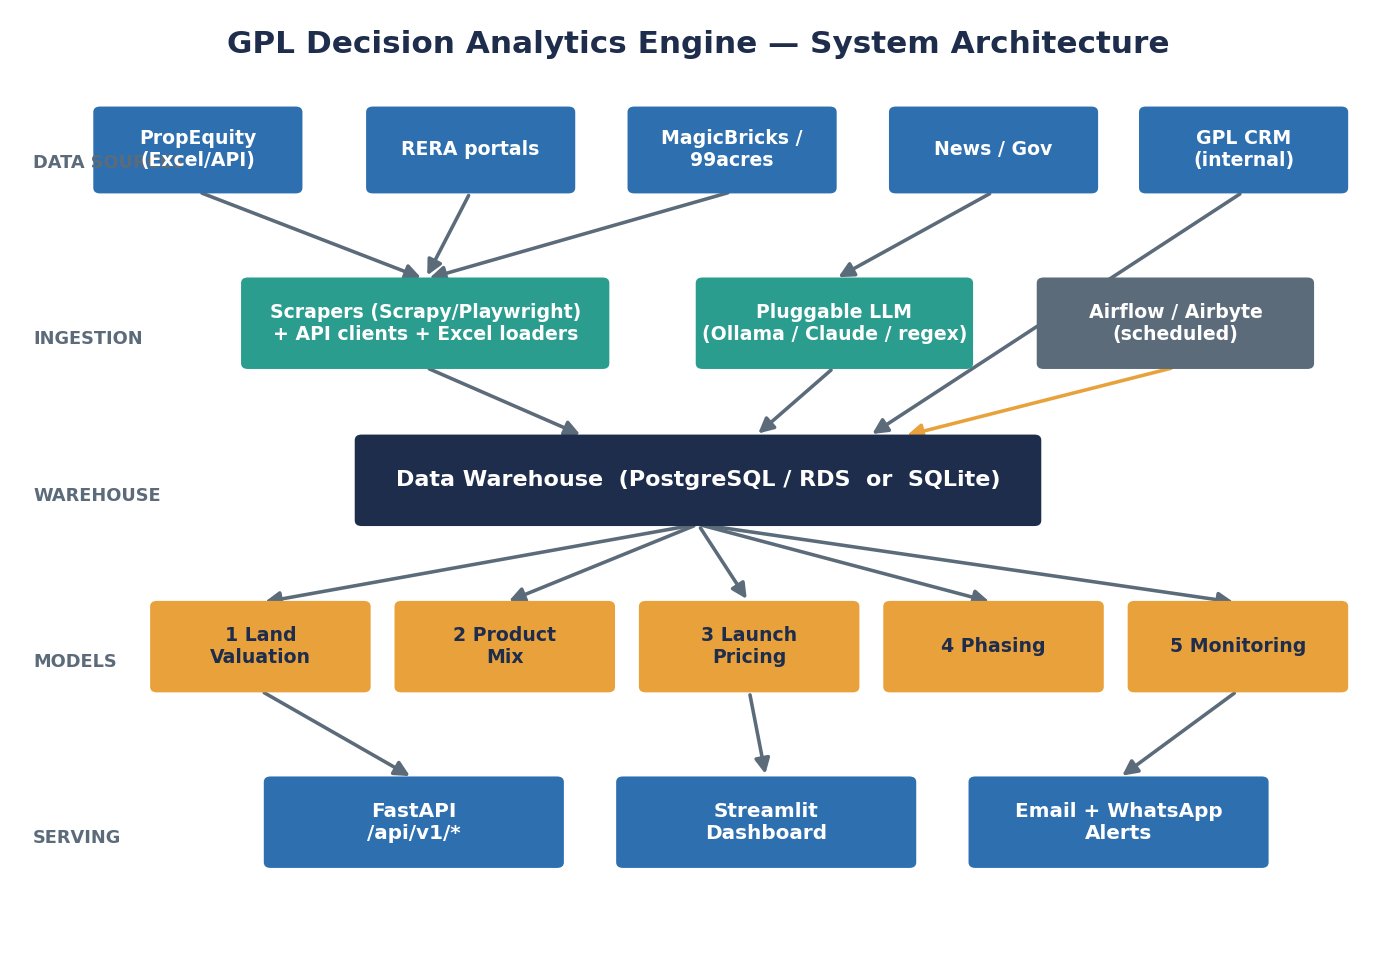
\includegraphics[width=\textwidth]{diagrams/architecture.png}
\caption{System architecture: sources $\rightarrow$ ingestion $\rightarrow$ warehouse $\rightarrow$ models $\rightarrow$ serving.}
\end{figure}

\begin{figure}[h!]
\centering
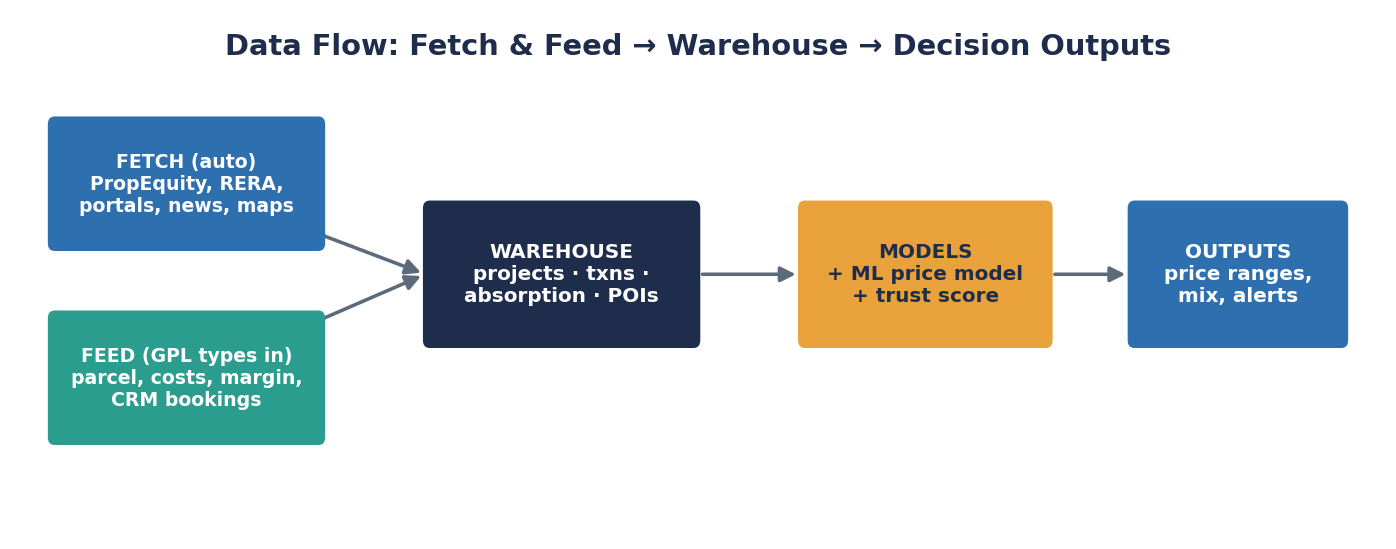
\includegraphics[width=\textwidth]{diagrams/data_flow.png}
\caption{Data flow: automatically fetched market data plus GPL-entered data feed one warehouse, which the models consume.}
\end{figure}

\subsection{Technology stack}
\begin{longtable}{p{3.2cm} p{5cm} p{5.5cm}}
\toprule
\textbf{Layer} & \textbf{Technology} & \textbf{Rationale} \\
\midrule
Warehouse & PostgreSQL / RDS (SQLite local) & Brief-permitted MVP choice; Snowflake-ready via \texttt{DATABASE\_URL}. \\
Structured ingest & Airbyte (self-hosted) + Python loaders & Open-source, no per-row pricing, data stays in GPL's environment. \\
Web scraping & Scrapy + Playwright & Static sites via Scrapy; JS portals via headless Chromium. \\
Modelling & scikit-learn, XGBoost, SciPy & Interpretable regression, non-linear price model, Monte Carlo. \\
LLM (text) & Ollama / Claude / regex (pluggable) & Self-hosted preferred; never receives GPL financial data. \\
Backend & FastAPI & Validated REST endpoints, auto OpenAPI docs. \\
Frontend & Streamlit & Rapid, polished internal dashboard. \\
Orchestration & Apache Airflow & Scheduled refresh with failure alerting. \\
Alerting & SendGrid + Interakt/Gupshup & Email + WhatsApp; console fallback offline. \\
\bottomrule
\end{longtable}

% ===================================================================
\section{Data Architecture \& Dictionary}
Data is either \textbf{fetched} automatically (\S3.1 of the brief) or \textbf{fed}
in by GPL teams (\S3.2). All of it lands in one warehouse, defined in
\texttt{db/schema.py}.

\subsection{Refresh schedule}
\begin{longtable}{p{4.5cm} p{4cm} p{2.5cm}}
\toprule
\textbf{Source} & \textbf{Method} & \textbf{Frequency} \\
\midrule
PropEquity & API / Excel import & Weekly \\
RERA portals (KA/MH/UP/TN) & API or scraper & Weekly \\
MagicBricks / 99acres & Playwright scraper & Daily \\
Google Maps (distances) & API (on demand) & Per parcel \\
News RSS & feedparser + LLM & Daily \\
Government announcements & scraper + LLM & Weekly \\
\bottomrule
\end{longtable}

\subsection{Core tables}
\begin{longtable}{p{3.3cm} p{4.5cm} p{5cm}}
\toprule
\textbf{Table} & \textbf{Key fields} & \textbf{Used for} \\
\midrule
\texttt{projects} & developer, lat/lng, units, sold, status & comparables, monitoring \\
\texttt{rera\_transactions} & config, carpet sqft, \textbf{price\_per\_sqft}, date & realisation, demand curve \\
\texttt{absorption\_snapshots} & quarter, units sold, avg price & demand curve, velocity \\
\texttt{points\_of\_interest} & category, lat/lng, planned & infrastructure score \\
\texttt{listings} & portal, listed psf, available units & price-change alerts \\
\texttt{land\_parcels} & lat/lng, area, FSI, BD notes & valuation inputs \\
\texttt{historical\_sales} & planned/sold, launch vs realised psf & GPL benchmark (CRM/SFDC) \\
\texttt{alerts}, \texttt{pipeline\_runs} & kind, severity, status & monitoring, health \\
\bottomrule
\end{longtable}

\noindent\textbf{Security (brief \S5.1):} GPL-internal data (costs, margins,
\texttt{historical\_sales}, CRM bookings) is \emph{never} sent to any external
LLM. The LLM layer only ever receives isolated text snippets (BD notes, news,
government announcements).

% ===================================================================
\section{Model Logic}
This section documents how each sub-module computes its output. Every result
object carries its inputs, intermediate scores, assumptions, and a trust score.

\subsection{Shared: comparable selection}
Transactions are comparable if within \texttt{radius\_km} (default 3\,km) and the
lookback window (24 months). Each is weighted by recency and similarity:
\[
w = \underbrace{\max\!\left(0.05,\,1-\tfrac{\text{months\_old}}{\text{lookback}}\right)}_{\text{recency}}
\times \underbrace{\big(0.6\,\text{dist\_sim} + 0.4\,\text{cfg\_sim}\big)}_{\text{similarity}}
\]
The weighted-average realisation is $\sum (p_i w_i)/\sum w_i$.

\subsection{Sub-module 1: Land Valuation}
\begin{figure}[h!]
\centering
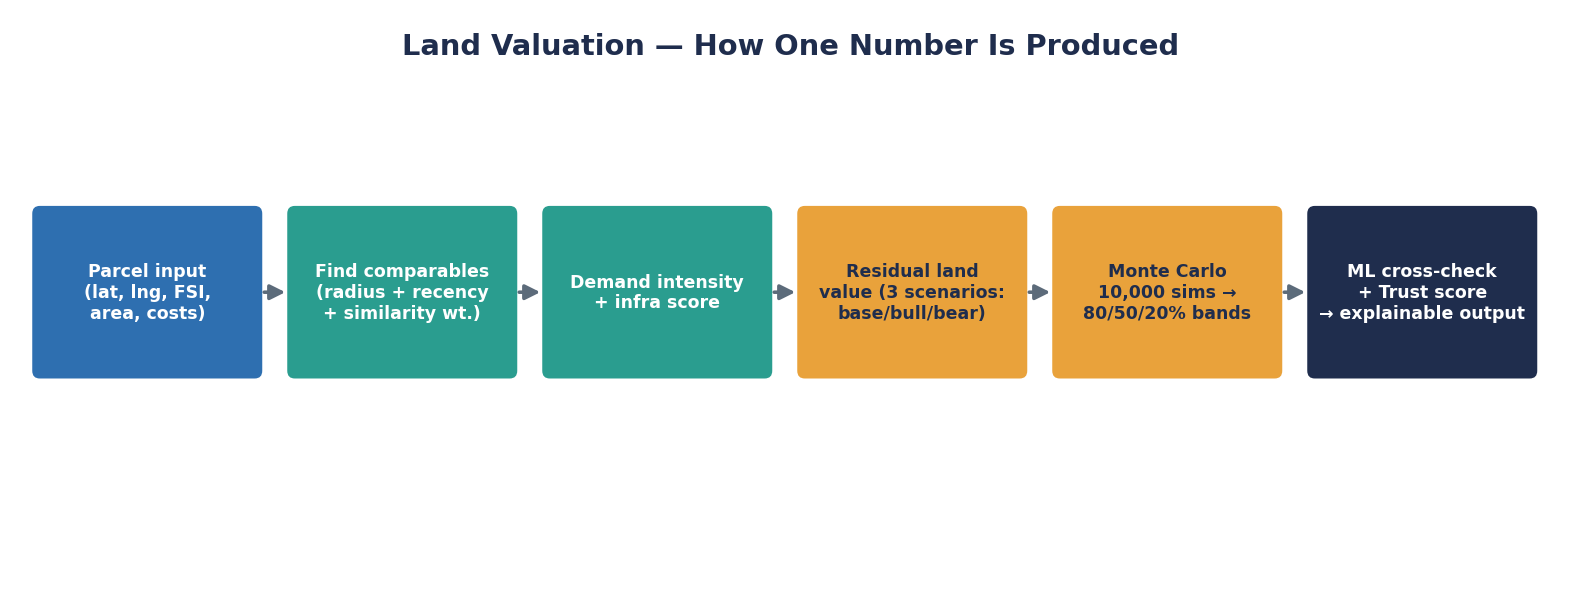
\includegraphics[width=\textwidth]{diagrams/valuation_pipeline.png}
\caption{How a single land-price recommendation is produced.}
\end{figure}

\textbf{Infrastructure score} (brief \S4.1) is a weighted sum of per-amenity
proximity scores (metro, IT-park, highway, school, hospital), weights
configurable per micro-market. \textbf{Residual land value} (brief \S4.2),
expressed per sqft of land area:
\[
\text{MaxLand} = \text{GDV} - \text{constr} - \text{finance} - \text{approvals} - \text{marketing} - \text{margin}
\]
computed for three scenarios (base $\times1.0$, bull $\times1.18$, bear
$\times0.85$ on realisation). A \textbf{Monte Carlo} of 10{,}000 simulations
(brief \S4.4) varies construction $\pm8\%$, realisation $\pm10\%$, absorption
$\pm25\%$ and reports the price supported at 80\%/50\%/20\% confidence.

\begin{lstlisting}[caption={Residual land value, per sqft of land (excerpt, \texttt{models/land\_valuation.py}).}]
saleable_per_land = fsi * saleable_ratio
gdv_per_land      = realisation_psf_saleable * saleable_per_land
construction      = construction_psf * fsi
finance           = construction * finance_rate * (duration/12) * avg_outstanding
margin            = gdv_per_land * min_margin_pct
max_land_psf_land = (gdv_per_land - construction - finance
                     - approvals*fsi - marketing*fsi - margin)
\end{lstlisting}

\subsection{Sub-module 2: Product Mix Optimiser}
A linear program over configuration area-shares $x_i$ maximises revenue density
subject to the FSI/saleable-area budget, with demand-gap-informed bounds so the
mix favours under-served, faster-selling configurations:
\[
\max \sum_i x_i \frac{\text{rev\_per\_unit}_i}{\text{sqft}_i}
\quad\text{s.t.}\quad \sum_i x_i = 1,\;\; 0.05 \le x_i \le \min(0.6,\,0.5 + 1.5\,\text{gap}_i)
\]

\subsection{Sub-module 3: Launch Pricing}
We fit a demand curve (units/month vs price) on comparables within 5\,km / 36
months, trying \textbf{linear, quadratic and exponential} forms and keeping the
best by $R^2$. Price is normalised to the local median so we compare
like-with-like across segments. The optimal price maximises
$\text{price}\times\text{velocity(price)}$ subject to cash-flow and
time-to-sellout constraints. Below five comparables the model flags sparse data
rather than presenting false precision (brief \S4.3).

\begin{lstlisting}[caption={Best-fit demand-curve selection (excerpt, \texttt{models/launch\_pricing.py}).}]
def fit_demand_curve(prices, vels):
    candidates = []
    for deg, name in ((1, "linear"), (2, "quadratic")):
        coef = np.polyfit(prices, vels, deg)[::-1]
        pred = np.vander(prices, deg+1, increasing=True) @ coef
        candidates.append(DemandCurve(name, r2_score(vels, pred), ...))
    # exponential: log(v) = a + b*price
    ...
    return max(candidates, key=lambda c: c.r2)   # keep the best shape
\end{lstlisting}

\subsection{Sub-module 4: Phased Inventory Release}
Each unit gets a saleability score (floor, facing, amenity, configuration,
price). Units split into \emph{phase-1} (launch to set the price anchor),
\emph{mid}, and \emph{premium} (held until $\ge40\%$ absorption, then released at
a 12--18\% premium, brief \S2.4). Phases map to the construction drawdown schedule.

\subsection{Sub-module 5: Competitive Monitoring}
Scans the warehouse and raises alerts: new RERA filings within 3\,km of a GPL
project, competitor price moves $\ge5\%$, absorption tightening ($\ge80\%$ sold)
or stalling, and government infrastructure announcements. Alerts are delivered by
email and WhatsApp (console fallback when unconfigured).

\subsection{ML price model \& trust score}
Alongside the comparable average, a gradient-boosted model
(\textbf{XGBoost}, scikit-learn fallback) learns price/sqft from location,
configuration, size, absorption, infrastructure and micro-market. It reports
\textbf{cross-validated $R^2$ and MAE} and acts as an independent cross-check:
close agreement raises confidence, a large gap is flagged for investigation.
Every module attaches a 0--1 \textbf{trust score} (sample size + price dispersion
+ model fit) banded HIGH/MEDIUM/LOW with plain-English reasons, so no number is
presented with false authority.

% ===================================================================
\section{API Documentation}
The FastAPI service (\texttt{api/main.py}) exposes every module; interactive
OpenAPI docs are auto-generated at \texttt{/docs}. All inputs are validated;
impossible values (e.g.\ FSI $>6$, negative margin) return HTTP 422.

\begin{longtable}{p{5.5cm} p{7cm}}
\toprule
\textbf{Endpoint} & \textbf{Purpose} \\
\midrule
\texttt{POST /api/v1/land-valuation} & 3-scenario land price + Monte Carlo + trust \\
\texttt{POST /api/v1/product-mix} & optimal configuration mix + revenue \\
\texttt{POST /api/v1/launch-pricing} & optimal price + escalation schedule \\
\texttt{POST /api/v1/launch-pricing/simulate} & test a price $\rightarrow$ velocity, sellout \\
\texttt{POST /api/v1/phasing} & release phases + triggers + cash-flow \\
\texttt{POST /api/v1/monitoring/scan} & run competitive scan \\
\bottomrule
\end{longtable}

\begin{lstlisting}[language=bash, caption={Example request.}]
curl -X POST http://localhost:8000/api/v1/land-valuation \
  -H 'Content-Type: application/json' \
  -d '{"lat":12.9010,"lng":80.2279,"area_acres":3.0,"fsi":2.5}'
\end{lstlisting}

% ===================================================================
\section{Deployment Guide}
The engine runs entirely within GPL's own AWS (or Azure) environment --- it is
not a SaaS and no GPL data is stored on developer servers.

\subsection{Local / evaluation}
\begin{lstlisting}[language=bash]
python3 -m venv .venv && source .venv/bin/activate
pip install -r requirements.txt
python -m ingestion.propequity_excel "<propequity .xlsx files>"
streamlit run dashboard/app.py        # dashboard
uvicorn api.main:app --reload         # API
\end{lstlisting}

\subsection{AWS production}
RDS PostgreSQL (encryption at rest, AES-256) behind the engine via
\texttt{DATABASE\_URL}; FastAPI on EC2 behind an ALB terminating TLS 1.3;
Streamlit on EC2; Airflow on MWAA; secrets in AWS Secrets Manager. The
security checklist and full steps are in \texttt{docs/DEPLOYMENT.md}.

% ===================================================================
\section{User Guide}
Open the dashboard and pick a module from the sidebar.

\subsection{Entering a land parcel}
In \textbf{1 $\cdot$ Land Valuation}: select the micro-market, enter latitude/
longitude, area (acres) and FSI, optionally adjust construction cost and minimum
margin, then click \textbf{Run valuation}. Impossible inputs are rejected with a
clear message.

\subsection{Interpreting outputs}
\begin{itemize}[noitemsep]
  \item \textbf{Base / Bull / Bear} --- the justifiable land price per sqft and total in  Rs.\,Cr.
  \item \textbf{Monte Carlo bands} --- use the 80\% number as a safe negotiation floor; the gap to 20\% is your upside room.
  \item \textbf{Confidence badge} (\textcolor{teal}{HIGH} / amber MEDIUM / red LOW) --- tells you how reliable the answer is and why.
  \item \textbf{ML cross-check} --- an independent model's price; close agreement = trust, a big gap = investigate.
  \item \textbf{Why} section --- the comparables, scores and assumptions behind every number.
\end{itemize}

\subsection{Adjusting assumptions}
Per-parcel cost and margin are editable in the sidebar; per-micro-market defaults
(infra weights, costs) are managed on the Admin page. If a recommendation looks
wrong, open the \textbf{Why} section --- it usually traces to an assumption you
can correct.

% ===================================================================
\section{Admin Guide}
\subsection{Adding a micro-market}
Micro-markets are created automatically when a PropEquity workbook is ingested.
To improve geocoding, add the locality to \texttt{MICROMARKET\_GEOCODES} in
\texttt{ingestion/propequity\_excel.py}; per-market infra weights and costs live
in the \texttt{micro\_market\_configs} table.

\subsection{Updating scrapers}
Selectors are isolated per source (\texttt{ingestion/scrapers/}). Update the CSS
selectors in the relevant scraper when a portal changes its markup.
MagicBricks/99acres are Cloudflare-protected --- in production route Playwright
through rotating residential proxies and scrape off-peak.

\subsection{Monitoring pipeline health}
The Admin page shows recent \texttt{pipeline\_runs} (status, record counts).
Airflow DAGs alert the admin by email + WhatsApp on any task failure within the
retry window. Ingesting new data automatically retrains the price model.

% ===================================================================
\section{Testing \& Verification}
The suite (\texttt{pytest}) covers all five sub-modules, input validation,
Monte Carlo determinism, the demand curve, the ML model and the trust score, on
an isolated seeded database. All tests pass; the dashboard and API are verified
end-to-end on the real ingested data (\textasciitilde1{,}000 projects,
1{,}700+ transactions across three cities, plus GPL's CRM bookings).

\vspace{1cm}
\begin{center}
{\color{navy}\rule{0.5\textwidth}{0.8pt}}\\[4pt]
\textit{Full source code, this documentation, and the markdown guides are
delivered in the project's private Git repository.}
\end{center}

\end{document}
